%--------------------------------------
%ELECTROTECHNIQUE - SCHEMA DE LIAISON A LA TERRE
%--------------------------------------

%utiliser les environnement \begin{comment} \end{comment} pour mettre en commentaire le préambule une fois la programmation appelée dans le document maître (!ne pas oublier de mettre en commentaire \end{document}!)

%\begin{comment}

\documentclass[a4paper, 11pt, twoside, fleqn]{memoir}

\usepackage{AOCDTF}

%--------------------------------------
%CANEVAS
%--------------------------------------

\newcommand\BoxColor{\ifcase\thechapshift blue!30\or brown!30\or pink!30\or cyan!30\or green!30\or teal!30\or purple!30\or red!30\or olive!30\or orange!30\or lime!30\or gray!\or magenta!30\else yellow!30\fi} %définition de la couleur des marqueurs de chapitre

\newcounter{chapshift} %compteur de chapitre du marqueur de chapitre
\addtocounter{chapshift}{-1}
	
\newif\ifFrame %instruction conditionnelle pour les couleurs des pages
\Frametrue

\pagestyle{plain}

% the main command; the mandatory argument sets the color of the vertical box
\newcommand\ChapFrame{%
\AddEverypageHook{%
\ifFrame
\ifthenelse{\isodd{\value{page}}}
  {\backgroundsetup{contents={%
  \begin{tikzpicture}[overlay,remember picture]
  \node[
  	rounded corners=3pt,
    fill=\BoxColor,
    inner sep=0pt,
    rectangle,
    text width=1.5cm,
    text height=5.5cm,
    align=center,
    anchor=north west
  ] 
  at ($ (current page.north west) + (-0cm,-2*\thechapshift cm) $) %nombre négatif = espacement des marqueurs entre les différents chapitres (à régler en fin de rédaction) (4.5cm vaut un espacement équivalement à la hauteur du marqueur, une page peut en contenir 6 avec cet espacement-la mais il est le plus équilibré)
    {\rotatebox{90}{\hspace*{.5cm}%
      \parbox[c][1.2cm][t]{5cm}{%
        \raggedright\textcolor{black}{\sffamily\textbf{\leftmark}}}}};
  \end{tikzpicture}}}
  }
  {\backgroundsetup{contents={%
  \begin{tikzpicture}[overlay,remember picture]
  \node[
  	rounded corners=3pt,
    fill=\BoxColor,
    inner sep=0pt,
    rectangle,
    text width=1.5cm,
    text height=5.5cm,
    align=center,
    anchor=north east
  ] 
  at ($ (current page.north east) + (-0cm,-2*\thechapshift cm) $) %nombre négatif = espacement des marqueurs entre les différents chapitres (à régler en fin de rédaction) (4.5cm vaut un espacement équivalement à la hauteur du marqueur, une page peut en contenir 6 avec cet espacement-la mais il est le plus équilibré)
    {\rotatebox{90}{\hspace*{.5cm}%
      \parbox[c][1.2cm][t]{5cm}{%
        \raggedright\textcolor{black}{\sffamily\textbf{\leftmark}}}}};
  \end{tikzpicture}}}%
  }
  \BgMaterial%
  \fi%
}%
  \stepcounter{chapshift}
}

\renewcommand\chaptermark[1]{\markboth{\thechapter.~#1}{}} %redéfinition du marqueur de chapitre pour ne contenir que le titre du chapitre %à personnaliser selon le nombre de chapitre dans le cours

%--------------------------------------
%corps du document
%--------------------------------------

\begin{document} %corps du document
	\openleft %début de chapitre à gauche

%\end{comment}

\begin{xltabular}{\textwidth}{c c X c c }
\caption{Différents types de DDR selon les composantes du courant de défaut}\\
\toprule
\thead{Type}		& \thead{Symbole}		& \thead{Caractéristiques}	& \thead{Forme d'onde}		& \thead{Type de charge} \\
\midrule
\endfirsthead %en-tête de la première page du tableau  
\multicolumn{5}{l}{\small\textit{Page précédente}} \\
\midrule %filet de milieu de tableau
\thead{Type}		& \thead{Symbole}		& \thead{Caractéristiques}	& \thead{Forme d'onde}		& \thead{Type de charge} \\
\midrule
\endhead
\midrule %filet de milieu de tableau
\multicolumn{5}{r}{\small\textit{Page suivante}} \\
\endfoot %pied de page de toutes les pages du tableau
\bottomrule
\endlastfoot %pied de page de la dernièredu tableau
Type AC		& \adjustbox{valign=t}{\includegraphics[height=0.4cm]{type_ac.png}}		& 
\begin{tabitemize}
\item détection des courants alternatifs résiduels 
\item utilisation courante en domestique couvrant la plupart des besoin 
\end{tabitemize}
&

\adjustbox{valign=t}{
\tikzset{every picture/.style={line width=0.75pt}} %set default line width to 0.75pt        
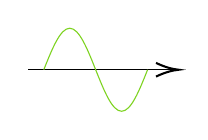
\begin{tikzpicture}[x=0.75pt,y=0.75pt,yscale=-1,xscale=1]
%uncomment if require: \path (0,131); %set diagram left start at 0, and has height of 131

%Straight Lines [id:da2943661507092279] 
\draw    (7.5,92.5) -- (78,92.5) ;
\draw [shift={(80,92.5)}, rotate = 180] [color={rgb, 255:red, 0; green, 0; blue, 0 }  ][line width=0.75]    (10.93,-3.29) .. controls (6.95,-1.4) and (3.31,-0.3) .. (0,0) .. controls (3.31,0.3) and (6.95,1.4) .. (10.93,3.29)   ;
%Shape: Wave [id:dp24323544196681968] 
\draw  [color={rgb, 255:red, 126; green, 211; blue, 33 }  ,draw opacity=1 ] (15,92.5) .. controls (19.08,82.25) and (22.98,72.5) .. (27.5,72.5) .. controls (32.02,72.5) and (35.92,82.25) .. (40,92.5) .. controls (44.08,102.75) and (47.98,112.5) .. (52.5,112.5) .. controls (57.02,112.5) and (60.92,102.75) .. (65,92.5) ;
\end{tikzpicture}}
 &
 
  \\
  
  
  Type A		& \adjustbox{valign=t}{\includegraphics[height=0.4cm]{type_a.png}}		& 
\begin{tabitemize}
\item détection des courants alternatifs résiduels et des courants continus pulsé
\item utilisation spécifique pour les charges électriques monophasées de type 1 
\end{tabitemize}
&

\adjustbox{valign=t}{
\tikzset{every picture/.style={line width=0.75pt}} %set default line width to 0.75pt        

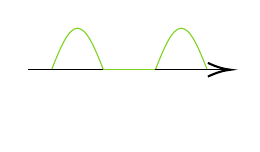
\begin{tikzpicture}[x=0.75pt,y=0.75pt,yscale=-1,xscale=1]
%uncomment if require: \path (0,108); %set diagram left start at 0, and has height of 108

%Shape: Wave [id:dp27700594343461393] 
\draw  [color={rgb, 255:red, 126; green, 211; blue, 33 }  ,draw opacity=1 ] (35,45) .. controls (39.08,34.75) and (42.98,25) .. (47.5,25) .. controls (52.02,25) and (55.92,34.75) .. (60,45) .. controls (64.08,55.25) and (67.98,65) .. (72.5,65) .. controls (77.02,65) and (80.92,55.25) .. (85,45) .. controls (89.08,34.75) and (92.98,25) .. (97.5,25) .. controls (102.02,25) and (105.92,34.75) .. (110,45) ;
%Shape: Rectangle [id:dp7690910497329457] 
\draw  [draw opacity=0][fill={rgb, 255:red, 255; green, 255; blue, 255 }  ,fill opacity=1 ][line width=5.25]  (32.5,45) -- (112.5,45) -- (112.5,67.5) -- (32.5,67.5) -- cycle ;
%Straight Lines [id:da5910455205676639] 
\draw    (23.75,45) -- (119.25,45) ;
\draw [shift={(121.25,45)}, rotate = 180] [color={rgb, 255:red, 0; green, 0; blue, 0 }  ][line width=0.75]    (10.93,-3.29) .. controls (6.95,-1.4) and (3.31,-0.3) .. (0,0) .. controls (3.31,0.3) and (6.95,1.4) .. (10.93,3.29)   ;
%Straight Lines [id:da5095890041059973] 
\draw [color={rgb, 255:red, 126; green, 211; blue, 33 }  ,draw opacity=1 ]   (60,45) -- (85,45) ;
\end{tikzpicture}}
 &
 

  \\
  
  
\end{xltabular}


\end{document}

